\documentclass[12pt,letterpaper]{article}
\usepackage{graphicx}
\usepackage{multirow}
\usepackage{authblk}
\usepackage{float}
\usepackage{rotating}
\usepackage{url}
\usepackage{lscape}
\usepackage{longtable}
\usepackage{subfigure}
\usepackage{natbib}
\usepackage{lineno}
\usepackage{amsmath,amsthm}
\usepackage[ruled,vlined,commentsnumbered]{algorithm2e}
%\usepackage{fullpage}	
\usepackage{anysize}
\marginsize{1.0in}{1.0in}{1.0in}{1.0in}
\linespread{1.6}

\newcommand{\Pic}[2][0.85]{\begin{center}\includegraphics[width=0.8\textwidth,height=#1\textheight,keepaspectratio]{#2}
 \end{center} }


\title{ A multiscale approach for hazard map construction}
\author[1]{ E. R. Stefanescu }
\author[1]{R. Shivaswamy}
\author[1]{A.K. Patra}
\author[2]{M. Bursik}
\affil[1]{Department of Mechanical and Aerospace Engineering, University at Buffalo, Buffalo, NY 14260}
\affil[2]{Department of Geology, University at Buffalo, Buffalo, NY 14260 }

\date{\today}


\begin{document}
\linenumbers
\maketitle

\begin{abstract}
To be added
\end{abstract}

\section{Introduction}
 
Three main processes are required in order to construct a simulation based probabilistic hazard map for volcanic 
debris: a) a good physical model, i.e. a simulator, with error control; b) an approach to uncertainty 
quantification usually involving an ensemble of simulator runs and an easily sampled  surrogate model; c) a multiscale process to analyze the simulator 
output into a map of the probability that some hazard criteria will be met.
The above processes lead to large amount of data and  CPU  intensive computing. This work advances state 
of the art in the last area, by deploying a novel programming model; and also by using a hierarchical approach in creating a fast surrogate of the simulator.
Handling the huge amount of data and computing is a primary concern in constructing a hazard map on distributed memory platforms. We describe a framework that we built using 
Hadoop to parallelize the data and compute intensive operations. We make use of Hadoop�s MapReduce framework 
to improve the speed of hazard map creation.
 For the purpose of this paper, we will assume that a suitable physical model of geophysical mass flow is available 
(TITAN2D).  Any simulator will naturally require values for certain input parameters. If the input values for a 
future event of interest were known exactly, then a hazard map could be generated from a single simulation 
evaluated at those inputs. Since we lack perfect knowledge of the future, it is necessary to examine flow behavior
over a range of inputs. While there are some sampling methods, such as Monte Carlo, that are \textit{nominally independent}
of the number of dimensions, there are far too expensive to use to create a feasible hazard map. 
The solution we came up to this problem can be summarized as:
\begin{itemize}
\item Running a \textit{relatively} small number of simulations (a few hundred to a few thousand) followed by
\item Constructing a meta-model (a model of the simulator) to act as a fast surrogate for the expensive simulator, and then
\item Generating the hazard map from the fast surrogate. 
\end{itemize}
In this work we introduce a multi-resolution scheme for an emulator construction on a high-dimensional parameter space. The 
proposed scheme overcomes some limitations of the 
parameter selection in the Bayesian emulator, which always  involves  repeated  inversion  of  error ``correlation  matrix",  $R$. 
The requirement  of  matrix  inversion  restricts  emulators  to  small  amounts  of  data mostly because for ``large" $N$:  $R$ is 
poorly conditioned and cost  of  inverting  matrix  is  $\mathcal{O}(N^3)$ operations.
Our scheme is based on mutual distances between data points and on a continuous extension of Gaussian functions. It uses a corse-to-fine hierarchy of the multi-resolution decomposition of a Gaussian kernel.
It generates a sequence of approximations at the given function on the data, as well as their extensions to any
newly-arrived data point. The subsampling is done by interpolative decomposition of the associated Gaussian kernel matrix in each scale in the hierarchical procedure. In this way a well-conditioned basis is identified and used in the extension/ extrapolation process. 


\section{Computational challenages}
A hazard map, as stated here, is a predictive map for a region  
which provides a probabilistic measure of
a hazard (e.g. geophysical flow reaching certain depths that can be considered hazardous/critical).
Simple uncertainty quantification using a Monte Carlo approach for generating such hazard maps will require $O(10^6)$ such simulations 
-- beyond current computational capabilities.
Since each flow simulation generates upwards of 2GB of data, a full ensemble with 2048 simulations generates almost 600GB of data which 
we have to then use to construct emulators. The computational difficulties include managing and accessing select entities 
from the large data and of processing it using compute intensive operations. Our approach to addressing these difficulties 
is to decouple the data mining and computationally intensive tasks through carefully crated workflows. 
We thus, employ the popular open source version of the Map-Reduce model, namely Hadoop, both in conjunction with a high performance cluster.
Problems involved in data extraction, movement over the 
network, and replication are addressed. The proposed computational methodologies also allow us to greatly improve the resolution of the 
developed hazard maps by using a hierarchical approach (rather than the simpler tessellation based localization used earlier \cite{keith}) 
allowing access to more data in the inference process and hence developing a more accurate localization of the covariance used in the hazard 
map construction.

\section{Multiscale emulator}
In the analysis of large scale simulations of complex dynamical systems, where the notion of time evolution comes into play, important problems 
are the identification of variables that capture the time evolution of the system. Traditionally, creating hazard maps has required detailed knowledge 
of past events which has been recorded in the volcano's geologic record. Knowledge of this history is frequently incomplete or even entirely unavailable.
Our goal is to produce a map showing the probability that each East-North point has of being inundated by a volcanic landslide with a flow-depth greater than a critical threshold from a collection of simulator runs whose parameters are drawn from a distribution that represents a volcanologist's best guess of the range of possible scenarios. We consider a study case for Soufri\`ere Hills, Montserrat, for which ranges of the flow volume, bed friction, internal friction and direction are available.
The 4-dimensional input parameter space is sampled using a simple space filling design like Latin Hypercube Design (LHD) to obtain 2048 sets of input. Simulations are performed at each sample point using the TITAN2D model to generate a map of maximum pile height, $h_{max}(\textbf{x})$ as function of position.
If we plot the maximum pile height at a specific location in space for each sample point we can easily observe the binning introduced by the LHD sampling (Fig.~\ref{fig_lhs} - blue dots). In LHD, each random direction (random variable or input) is divide into $N_{bin}$ bins of equal probability and one random value is selected in each bin \cite{mckay1979comparison}. 
\begin{figure}
\begin{center}
%\resizebox*{15cm}{!}{\includegraphics{net_flow.pdf}}
\resizebox*{9cm}{!}{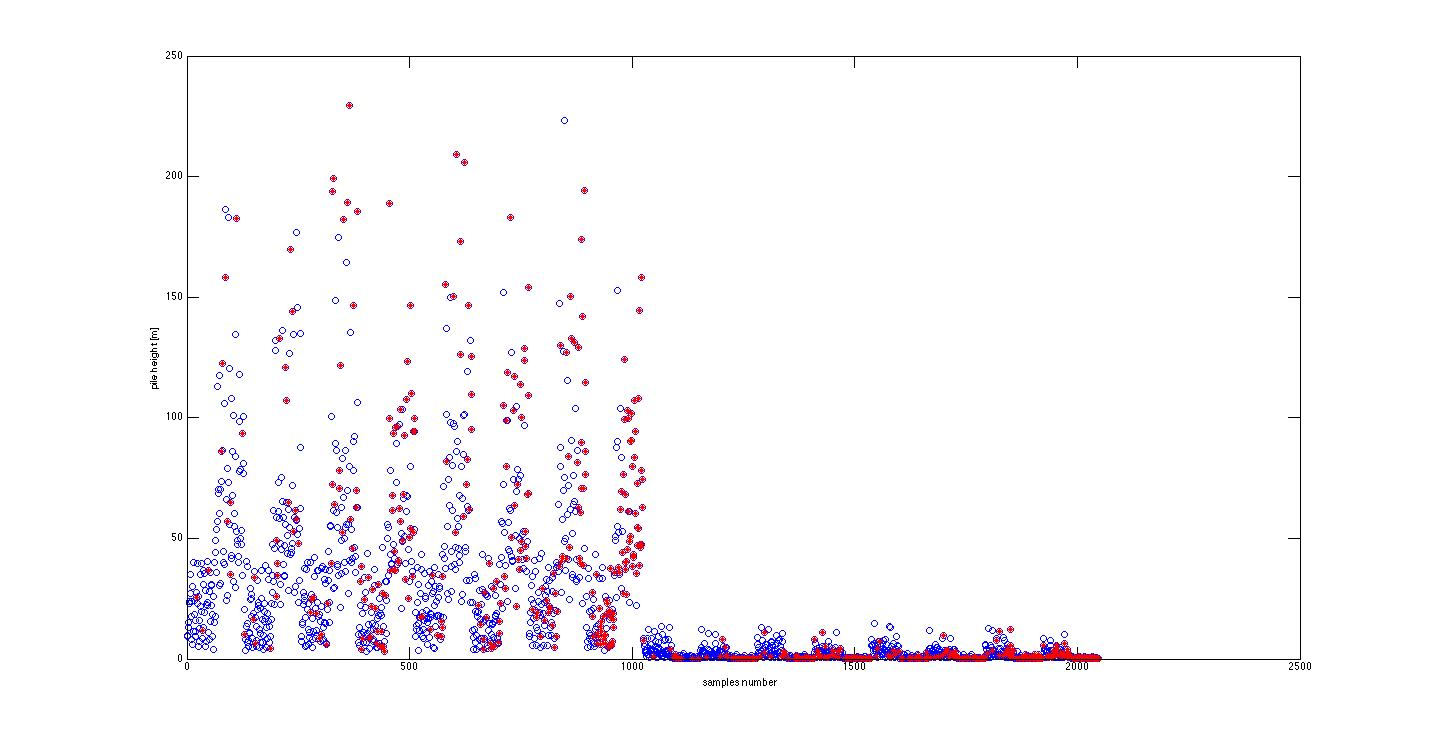
\includegraphics{figs/lhs_hmax.jpg}}
\vspace{-30pt}
\caption{\label{fig_lhs} Blue dots represent the maximum pile heigh at a selected location for each LHD sample point, the red starts represent the multiscale data samples.}
\end{center}
\end{figure}
By performing a multiscale data sampling we identify a well-conditioned basis of a low rank Gaussian kernel matrix, used in identifying scattered data sampling (Fig.~\ref{fig_lhs} - red stars). Using the obtained sample data, $h_{max}$ is evaluated at re-sample points.

Typical usage involves evaluating the fast surrogate at hundreds of thousands or millions of re-sample input points. The number of samples needed to generate the fast surrogate are exponential in the number of dimensions. This effectively limits its application to when there are three or fewer uncertain dimensions. This implies that we need to change the representation of the 2048 data sets, into a low-dimensional that describe the data in a faithful manner. In order to achieve this goal, we use a technique that relies on graph-based algorithms. Weighted graphs are employed to represent the ``geometry" based on the local similarity or interaction between the data points. Since each of the data sample is represented by a collection of numerical attributes, the condition of two nodes to be connected is based on the proximity of the corresponding data points in the feature space.

A graph $G=(V,E)$ is characterized by a set of vertices $V=\{1,\dots,m\}$ and a set of edges $E=\{e_{ij}|i,j \in V\}$.
Let $A=[a_{ij}]$ be the $m\times m$ adjacency matrix such that $a_{ij}$ represents the weight of edge $e_{ij}$. If there is no edge between vertices $i$ and $j$ then $a_{ij}=0$.
Clustering the vertices $V$ into $c$ disjoints sets $V_1, \dots, V_c$ with $m_i=|V_i|$, the adjacency matrix will have
the following form:
\begin{equation}
A_{m,n} =
 \begin{bmatrix}
  A_{11}  & \cdots & A_{1c} \\
  A_{2,1} & \cdots & A_{2,n} \\
  \vdots  & \ddots & \vdots  \\
  A_{c1}  & \cdots & A_{c,c}
 \end{bmatrix}
\end{equation}
where each diagonal block $A_{ii}, i=1,\dots,c$, is an $m_i \times m_i$ matrix that can be considered as a local
adjacency matrix for cluster $i$. The off-diagonal $m_i \times m_j$ blocks $A_{ij}$ with $i \neq j$, contain the
set of edges between vertices belonging to different clusters.

In a perfectly clusterable graphs, the off-diagonal blocks will not contain any edges, thus yielding $A_{ij}=0$,
and the graph will consist of $c$ disconnected components. In a realistic scenario, with a graph forming good clusters
most of the edges will be contained within the diagonal blocks $A_{ii}$, while the off-diagonal blocks $A_{ij}$ will
contain only a few edges.
The decay in the $A$'s spectrum is a measure of the connectivity of the points in the graph.
\begin{itemize}
\item One extreme case corresponds to the graph where all the all the nodes are disconnected. This leads to
$A$ being equal to the identity operator and thus to a flat spectrum.
\item Another case is the graph where all the nodes are connected to all the other nodes weights equal to
$1$. In this case, $A$ has one eigenvalue equal to 1, and all other eigenvalues are equal to 0 (we obtain the
fastest decay possible for the a diffusion operator).
\item Usually the spectrum of the heat kernel decays smoothly. 
\end{itemize}

Many dimensionality reduction methods involve a spectral decomposition of large matrices, whose dimensions are proportional to the size of the data, has high computational cost. The $n$ observations
${f_1,f_2,\dots, f_3}$ are considered the data points.
When the covariance of the data points is unknown, an artificial function has to be chose. A Gaussian covariance is a popular choice:
\begin{align}
g_{\epsilon}(x,x') = exp(- \parallel x-x' \parallel ^ 2 / \epsilon)
\end{align}
where $\parallel\dots\parallel$ constitutes a metric on the space (Euclidean distance in our case). The corresponding covariance (affinities) is
\begin{align}
(G_{\epsilon})=g_{\epsilon}(x_i,x_j), \; i,j=1,2,\dots,n.
\end{align}
The combination of clustering and low rank approximation gives a better approximation of the 
original graph. A standard low rank computation is likely to only extract information from the
largest or a few dominant clusters. 
The $Nystr\ddot{o}m$ method, vastly used for out-of-sample extension has three significant disadvantages: (a) Diagonalization of $G$ costs $\mathcal{O}(n^3)$ operations; (b) $G$ may be 
ill-conditioned due to fast decay of its spectrum, and (c) it is unclear how to choose the length parameter $\epsilon$ since the output is sensitive to the choice of $\epsilon$.
To overcome these limitations a multiscale approach is used: a sequence of Gaussian kernel matrices $G_s, s=0,1, \dots$, whose entries are $(G_{\epsilon})=g_{\epsilon}(x_i,x_j)$, where 
$\epsilon_s$ is a positive monotonic decreasing function of $s$, which tends to zero as the scale parameter $s$ tends to infinity (i.e. $\epsilon_s=2^{-s}$, $s=0,1,\dots$.). 

By the application of a randomized interpolative decomposition(ID) to $G_s$, a well-conditioned basis is identified for it numerical range. In each scale $f$ is decomposed into a sum of its 
projections on this basis and it is extended as $\bar{f}_{*} = G_{*}G^{-1}f$. In addition, selection of the proper columns in $G_s$ is equivalent to data sampling of the associated data points.

The method requires no grid. It automatically generates a sequence of adaptive grids according to the data distribution. It is based on the mutual distances between the data points and on a continuous 
extension of Gaussian functions. In addition, most of the costly computations are done just once during the process, independently of the number of the extended data points since they depend only in the data and on the given function. 

\begin{algorithm}
\SetAlgoLined
 \KwData{A data set $D=\{x_1,\dots,x_n\} \in \mathcal{R}^d$ (based on LHS design) }
 \KwResult{A function $f= [f_1,\dots,f_n]^T$}
 \While {$i \le n$}{
  Run TITAN2D simulation for each $x_i$. \\
  Use a downsample algorithm  $\rightarrow$ $N$ downsample points.\\
  For each $N$ generate an $f$ based on maximum height and apply the response surface calculation algorithm.\\
  Perform multiscale d
  
  
  }
\caption{Initial setup}
\end{algorithm}
  
\begin{algorithm}
 \SetAlgoLined
 \KwData{A data set $D=\{x_1,\dots,x_n\} \in \mathcal{R}^d$, $T>0$, a new data point $x_{*}\in \mathcal{R}^d$, a function $f= [f_1,\dots,f_n]^T$ to be
 extended and an error parameter $err \ge 0$. }
 \KwResult{An approximation $F=[F_1,\dots,F_n]^T$ of $f$ on $D$ and its extension $F_{*}$ to $x_{*}$ }
 Set the scale parameter $s=0$, $F^{(-1)}=0\in \mathcal{R}^n$ and $ F_{*}^{(-1)}=0$.\\
 \While{$\parallel f -F^{(-1)} \parallel > err$ }{
  Form the Gaussian kernel $G^{(s)}$on $D$ with $\epsilon_s=\frac{T}{2^s}$\;
  Estimate numerical rank $l^{(s)}$ of $G^{(s)}$\;
  Generate $A$ whose entries are i.i.d Gaussian random variables of zero mean and unit variance: $W=AG^{(s)}$\;
  Apply pivoted QR on $W$ $\rightarrow$ $WP_R=QR$\;
  Split R and Q st. \[
\left[
\begin{array}{c|c}
R_{11} & R_{12} \\
\hline
0 & R_{22}\\
\end{array}
\right]
\]
 and [ Q1 $\mid$ Q2] \;
    $S=Q_1R_{11}$ \;
    Columns of $S$ constitute a subset of of the columns of $W$. The corresponding columns of $G^{(s)}$ are collected into a matrix $B$,
    so that the column of $j$th column of $B^{(s)}$ is the $i_j$th column of $A$. The sampled dataset is $D_s$.\;
    Calculate the pseudo-inverse $(B^{(s)})^{\dagger}$ of $B^{(s)}$.\;
    Calculate the coordinates vector of the orthogonal projection of $f^{(s)}$ on the range of $B^{(s)}$ in the basis of $B^{(s)}$'s 
    columns $c=(B^{(s)})^{\dagger}f$\;
    Calculate the orthogonal projection of $f$ on the columns of $B^{(s)}$, $f^{(s)}=B^{(s)}c$\;
    Form the matrix $G^{(s)}_{*}=[g_{\epsilon}(x_*,x_{s_1}) \dots g_{\epsilon}(x_*,x_{s_{l^{(s)}}})]$\;
    Calculate the extension $f^{(s)}_* = G_{*}c$\;
    Set $F^{(s)}=F^{(s-1)} + f^{(s)}$, $F_{*}^{(s-1)}+f_{*}^{(s)}$, s=s+1\;
 }
 \caption{Response surface calculation}
\end{algorithm}

\bibliographystyle{plainnat} \bibliography{mybib}
\end{document}